\subsection{Interacciones y alcance del sistema: Diagrama de Contexto}
A continuación mostramos el Diagrama de Contexto de la empresa. En el mismo se detallan las interacciones entre los diversos agentes de la empresa y su interacción con el sistema propuesto:

\subsubsection{Diagrama}

\begin{figure}[H]
    \centering
    \includegraphics[width=\textwidth]{imagenes/contexto-con-sistema.png}
\end{figure}

\begin{figure}[H]
    \centering
    \includegraphics[width=\textwidth]{imagenes/contexto-sin-sistema.png}
\end{figure}

\newpage

\subsubsection{Observaciones}

Debido a la gran cantidad de interacciones entre los agentes decidimos, por una cuestión de comprensibilidad, separar el diagrama de contexto en dos partes complementarias. Por un lado se presentan las interacciones de todos los agentes con el Sistema a implementar. Por el otro, se muestran las acciones que suceden entre los demás agentes entre si. Estos diagramas no deben ser leídos por separado, sino que son dos partes del mismo, que representa el Diagrama de Contexto final entre todos los agentes.

Además, para evitar confusiones y reducir el espacio, cada vez que se daba el caso de que había múltiples flechas de interacción entre dos agentes, la simplificamos en una sola donde listamos todas las formas en las que un agente actúa sobre el otro. Por eso, hay múltiples líneas de texto en cada flecha y estas deben ser leídas como una flecha en sí por cada línea de texto.

\newpage

\subsection{Requerimientos del sistema: Diagrama de Objetivo}
En este diagrama detallamos como la implementación del sistema propuesto colaborará con la mejora de los procesos de la empresa.

\subsubsection{Objetivos principales}

\begin{figure}[H]
    \centering
    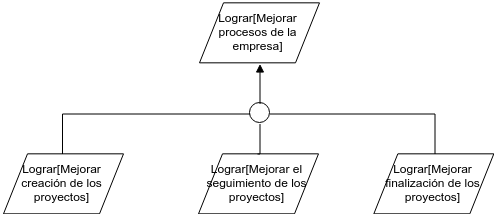
\includegraphics[width=\textwidth]{imagenes/objetivos-principales.png}
\end{figure}

\subsubsection{Creacion del proyecto}

\begin{figure}[H]
    \centering
    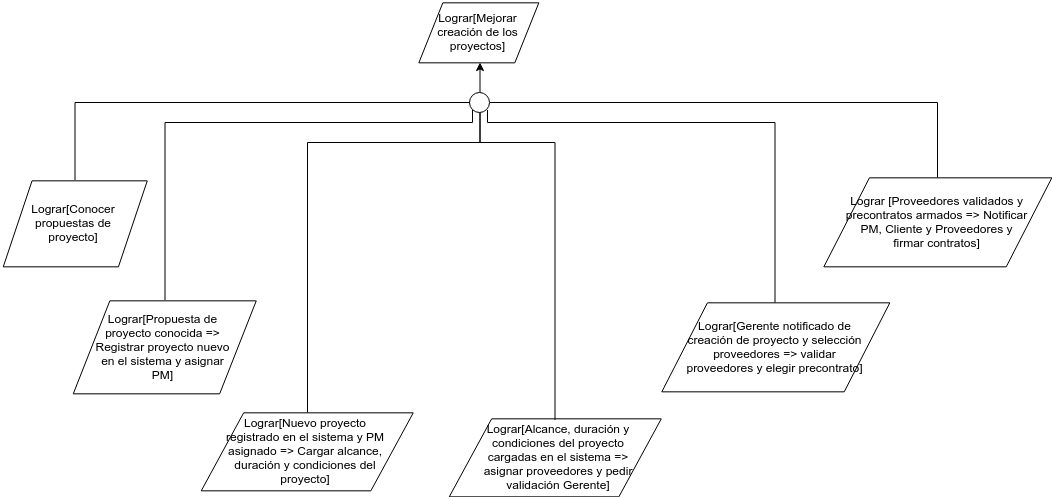
\includegraphics[width=18cm, keepaspectratio]{imagenes/objetivos-creacion-principal.png}
\end{figure}

\vspace{1em}

\begin{figure}[H]
    \centering
    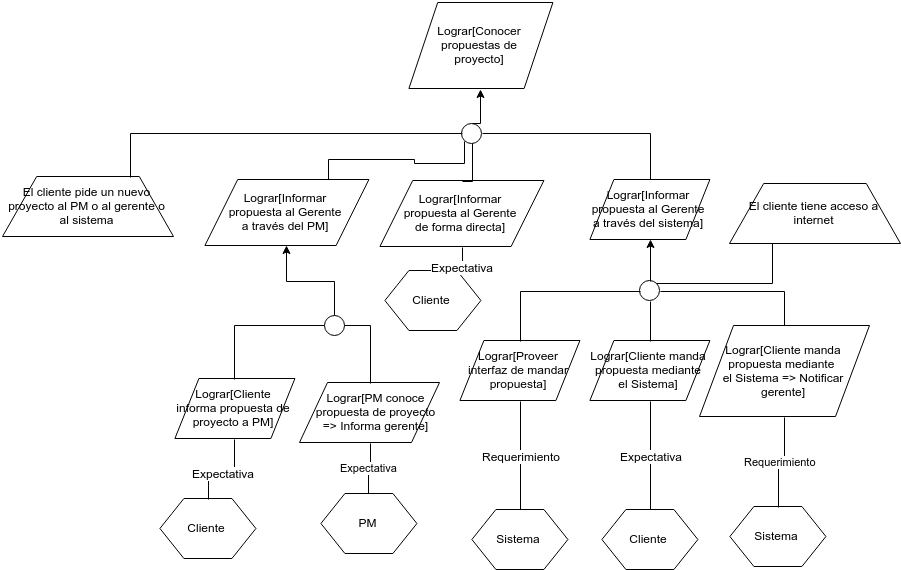
\includegraphics[width=\textwidth]{imagenes/objetivos-creacion-1.png}
\end{figure}

\vspace{1em}

\begin{figure}[H]
    \centering
    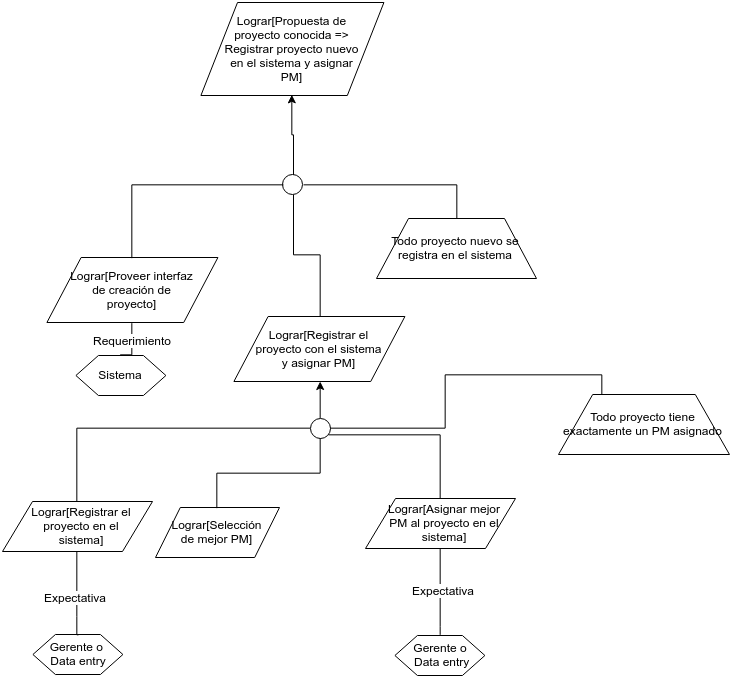
\includegraphics[width=\textwidth]{imagenes/objetivos-creacion-2.png}
\end{figure}

\begin{figure}[H]
    \centering
    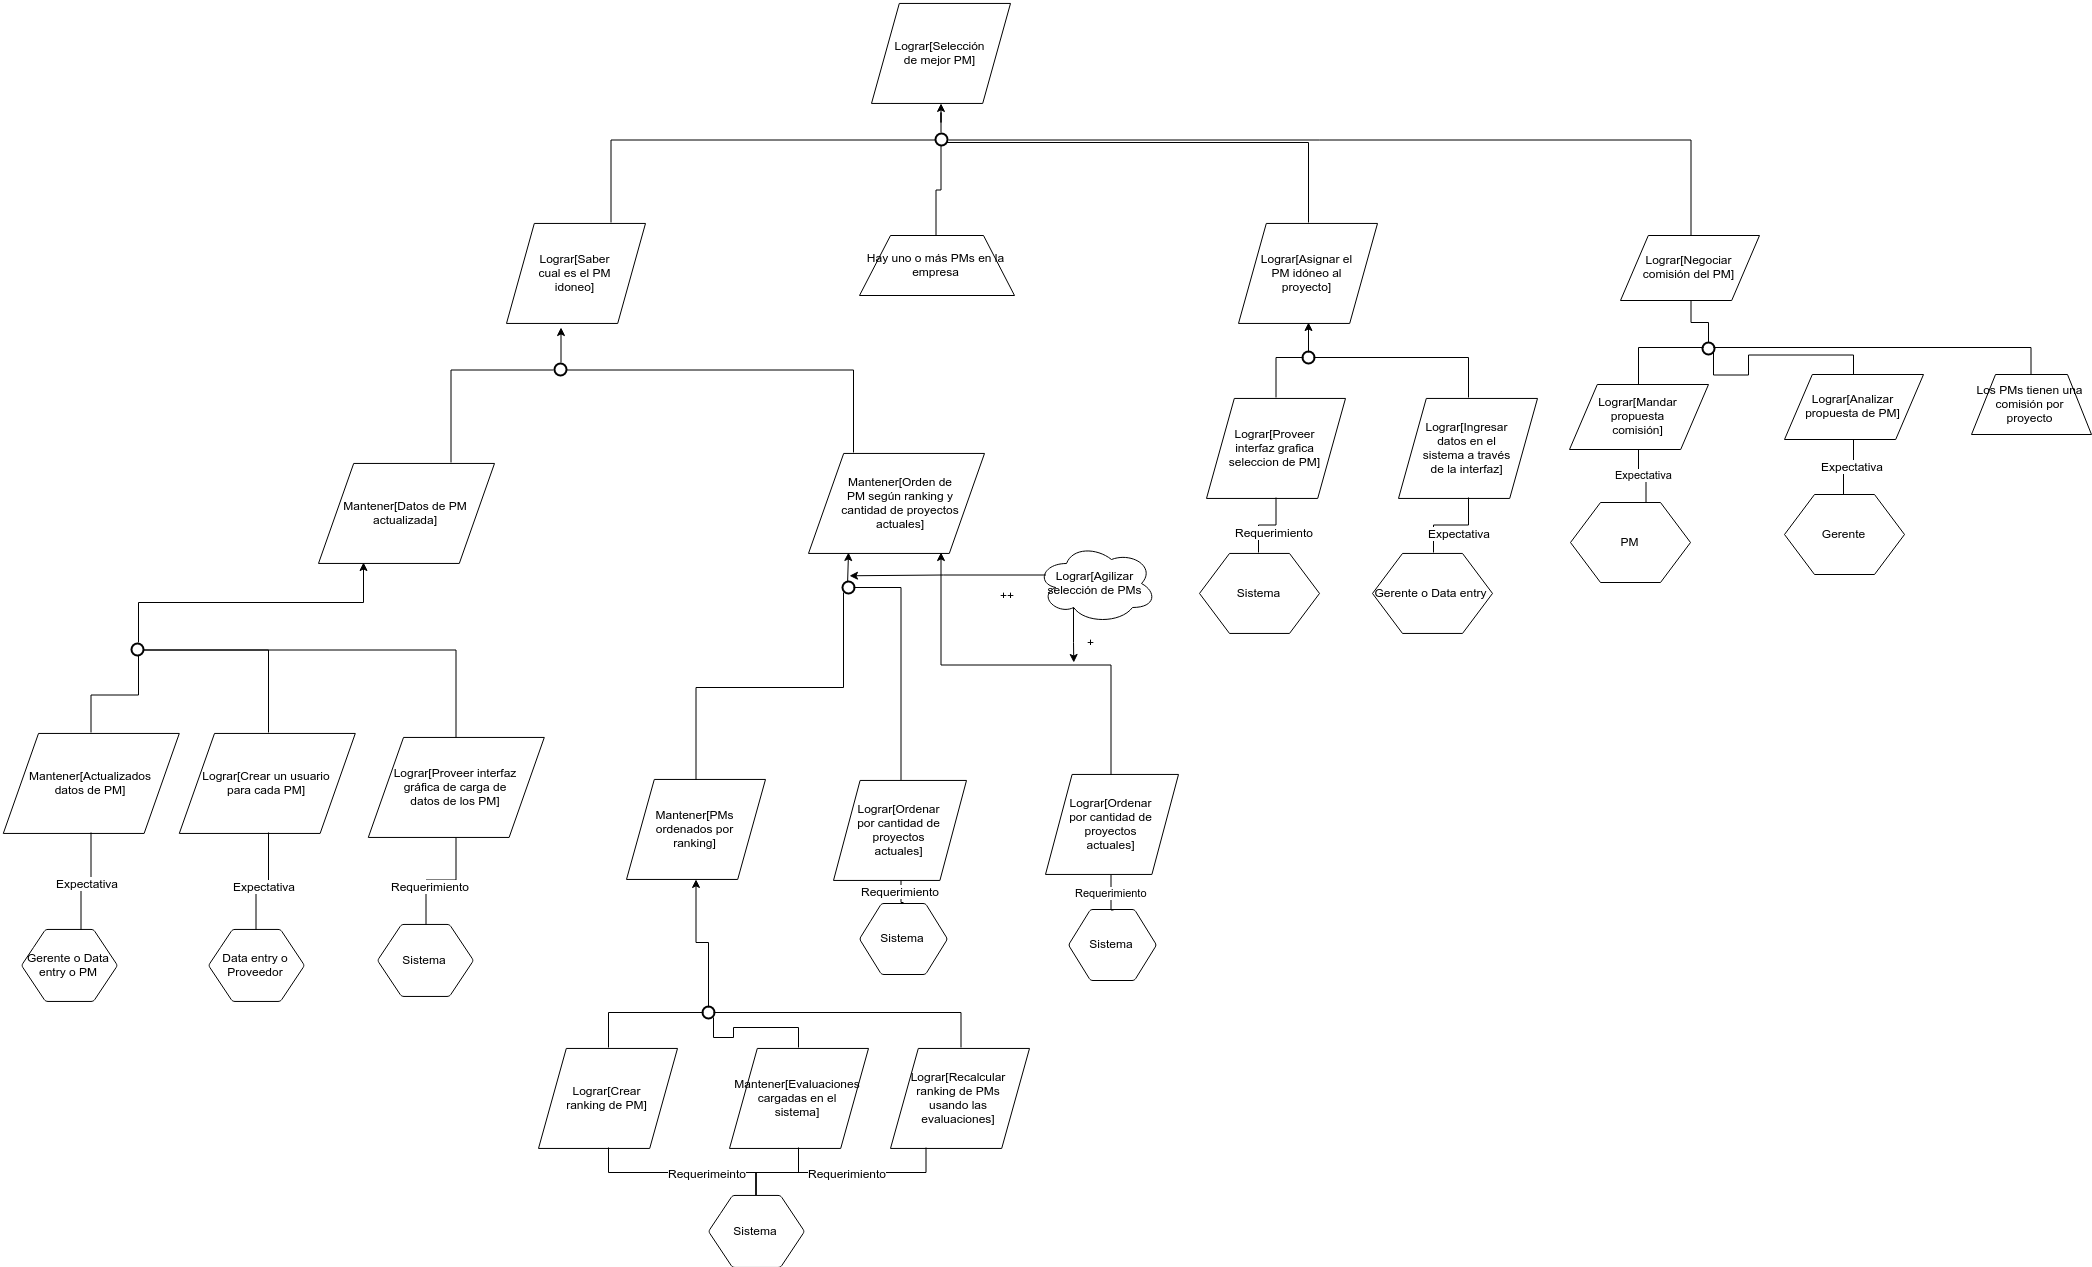
\includegraphics[width=10in, keepaspectratio, angle=90]{imagenes/objetivos-seleccion-mejor-pm.png}
\end{figure}

\subsubsection{Seleccion mejor proveedor}

\begin{figure}[H]
    \centering
    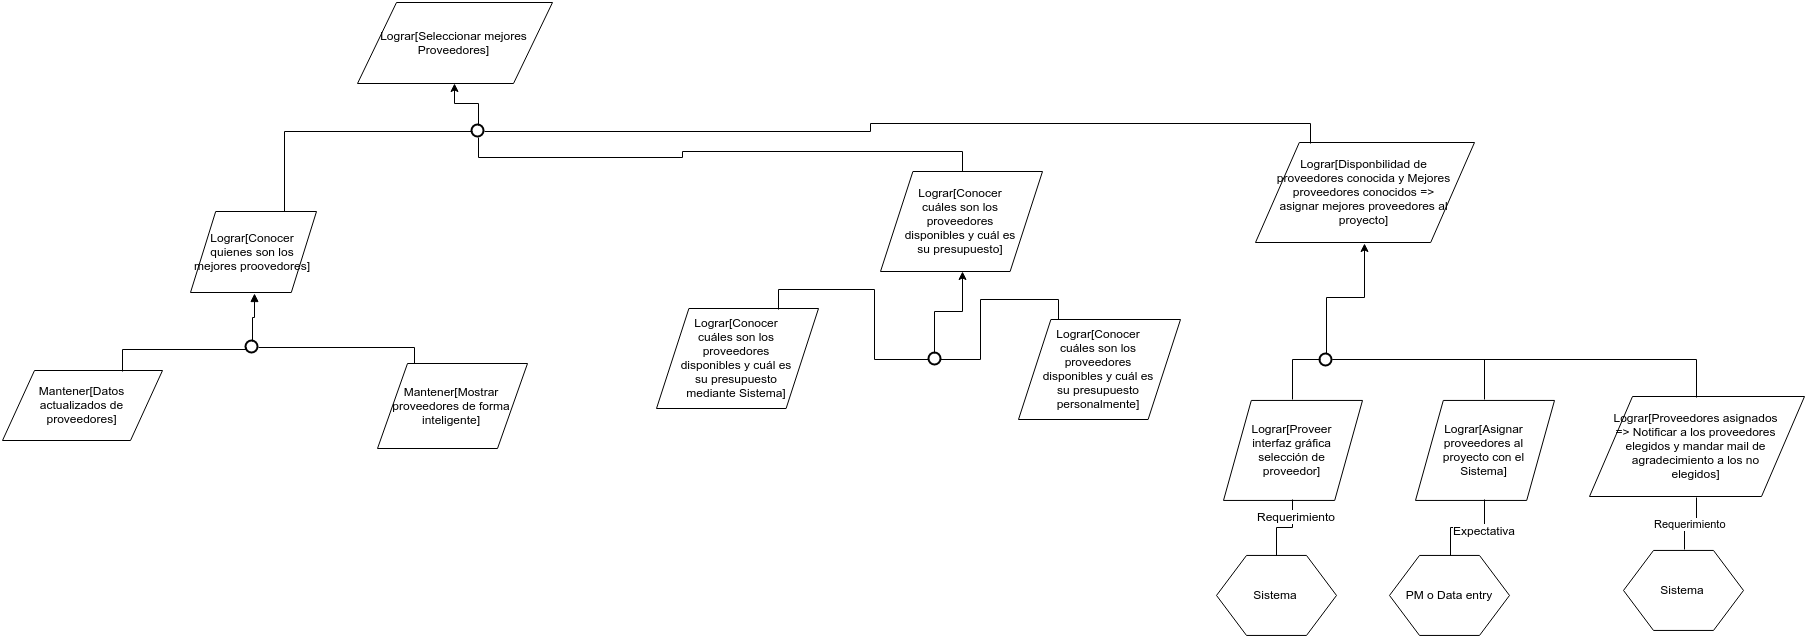
\includegraphics[width=9in, keepaspectratio, angle=90]{imagenes/objetivos-seleccion-mejor-proveedor-principal.png}
\end{figure}

\begin{figure}[H]
    \centering
    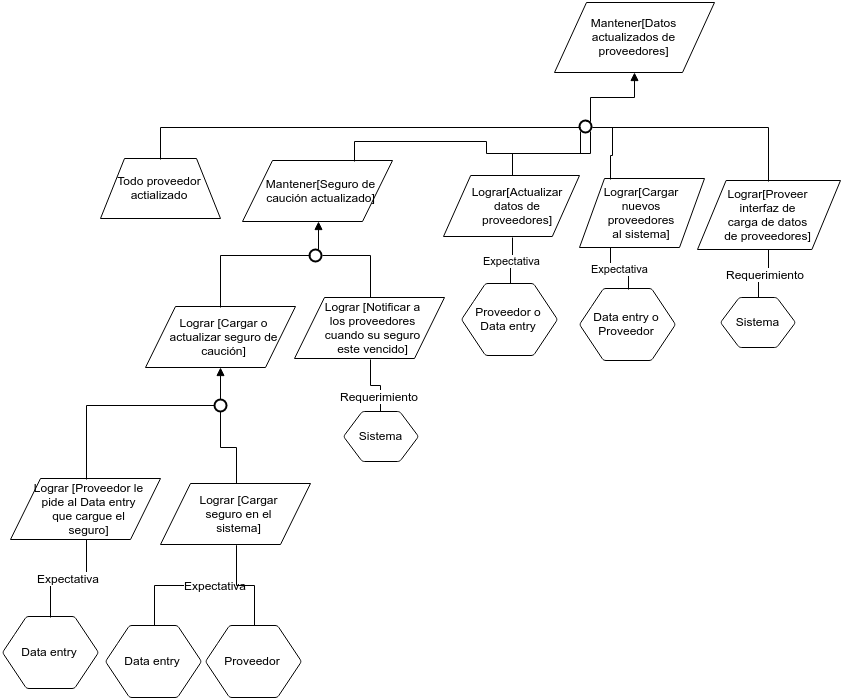
\includegraphics[width=\textwidth]{imagenes/objetivos-seleccion-mejor-proveedor-1.png}
\end{figure}

\begin{figure}[H]
    \centering
    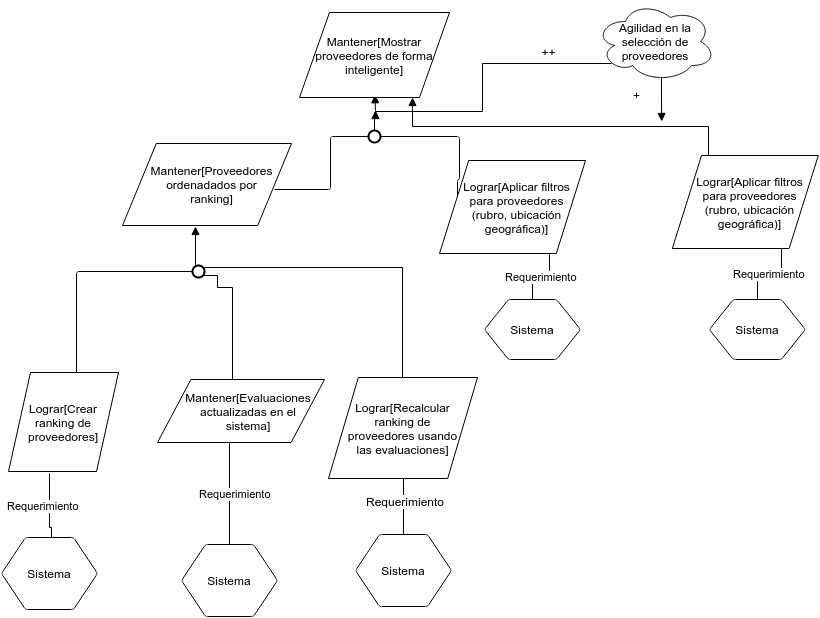
\includegraphics[width=\textwidth]{imagenes/objetivos-seleccion-mejor-proveedor-2.png}
\end{figure}

\begin{figure}[H]
    \centering
    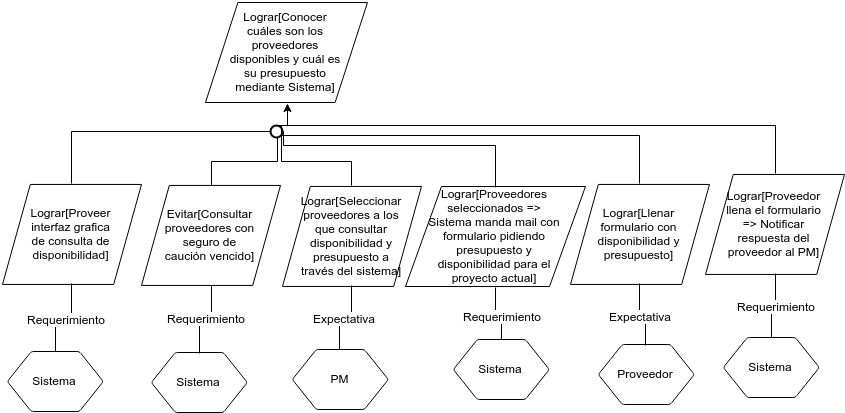
\includegraphics[width=\textwidth]{imagenes/objetivos-seleccion-mejor-proveedor-3.png}
\end{figure}

\begin{figure}[H]
    \centering
    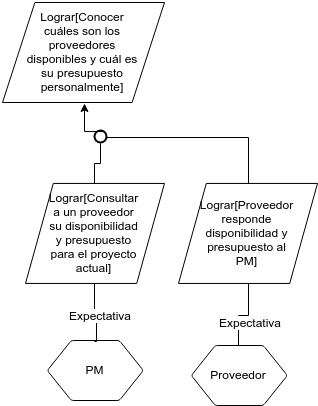
\includegraphics[width=.5\textwidth]{imagenes/objetivos-seleccion-mejor-proveedor-4.png}
\end{figure}

\subsubsection{Seguimiento del proyecto}

\includegraphics[width=\textwidth]{imagenes/seguimiento1.png}

En este grafico se muestran los niveles mas altos de 'Seguimiento de proyecto'. Aca no se ven los refinamientos de 'Mantener estado de proyectos actualizados', que estan en las siguientes figuras.

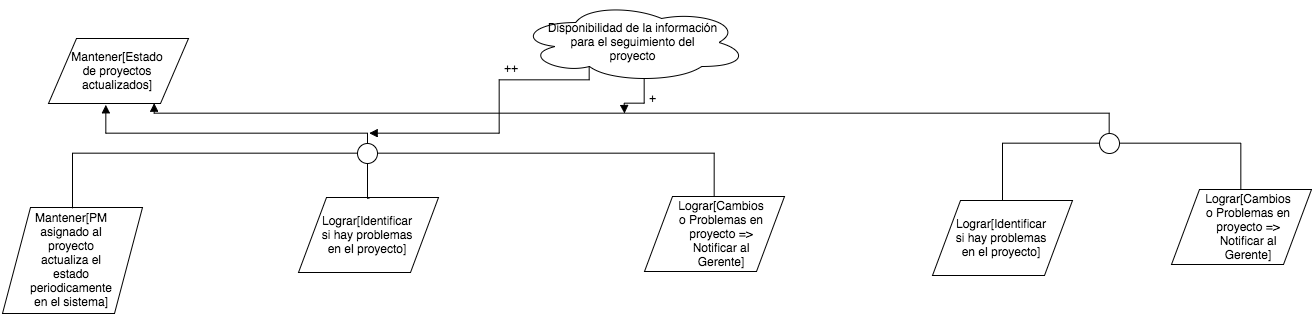
\includegraphics[width=\textwidth]{imagenes/seguimiento2.png}

En este desgloce, se puede apreciar un O-refinamiento en el cual las dos opciones tienen objetivos en comun pero uno agrega la opcion de mantener al PM actualizando obligatoriamente el estado de proyecto cada poco tiempo. Estos objetivos a su vez los desglozamos en las siguientes figuras.

\includegraphics[width=\textwidth]{imagenes/seguimiento3.png}

Aca se puede ver el Y-refinamiento de la primer alternativa.

\includegraphics[width=\textwidth]{imagenes/seguimiento4.png}

Este es el detalle de la segunda alternativa, muy similar a la primera pero con menos funcionalidad.

\newpage

\subsubsection{Finalizacion del proyecto}

\begin{figure}[H]
    \centering
    \includegraphics[width=9in, keepaspectratio, angle=90]{imagenes/objetivos-finalizacion-principal.png}
\end{figure}

\includegraphics[width=\textwidth]{imagenes/objetivos-finalizacion1.png}

\includegraphics[width=\textwidth]{imagenes/objetivos-finalizacion2.png}

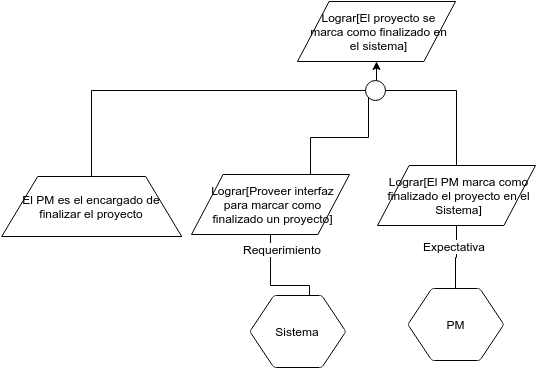
\includegraphics[width=\textwidth]{imagenes/objetivos-finalizacion3.png}

\includegraphics[width=\textwidth]{imagenes/objetivos-finalizacion4.png}

\includegraphics[width=\textwidth]{imagenes/objetivos-finalizacion5principal.png}

\includegraphics[width=\textwidth]{imagenes/objetivos-finalizacion51.png}

\includegraphics[width=\textwidth]{imagenes/objetivos-finalizacion52.png}

\includegraphics[width=\textwidth]{imagenes/objetivos-finalizacion53.png}

\newpage

\subsubsection{Observaciones}

El diagrama de objetivos se presenta con la idea de ser leído de izquierda a derecha. Frecuentemente, tratamos de colocar los objetivos que se suceden entre sí de esta forma para 'simular' los diferentes pasos que se suceden a través del tiempo.

Separamos el diagrama en varias partes (como el Diagrama de Contexto) varias veces debido al tamaño del mismo. Estos gráficos se deben leer como las diferentes partes de un mismo diagrama. Asi, presentamos primero las ramas superiores que engloban los objetivos de más alto nivel y luego mostramos como se va completando cada rama con su diagrama correspondiente.
